% Options for packages loaded elsewhere
\PassOptionsToPackage{unicode}{hyperref}
\PassOptionsToPackage{hyphens}{url}
%
\documentclass[
  man,floatsintext]{apa6}
\usepackage{amsmath,amssymb}
\usepackage{iftex}
\ifPDFTeX
  \usepackage[T1]{fontenc}
  \usepackage[utf8]{inputenc}
  \usepackage{textcomp} % provide euro and other symbols
\else % if luatex or xetex
  \usepackage{unicode-math} % this also loads fontspec
  \defaultfontfeatures{Scale=MatchLowercase}
  \defaultfontfeatures[\rmfamily]{Ligatures=TeX,Scale=1}
\fi
\usepackage{lmodern}
\ifPDFTeX\else
  % xetex/luatex font selection
\fi
% Use upquote if available, for straight quotes in verbatim environments
\IfFileExists{upquote.sty}{\usepackage{upquote}}{}
\IfFileExists{microtype.sty}{% use microtype if available
  \usepackage[]{microtype}
  \UseMicrotypeSet[protrusion]{basicmath} % disable protrusion for tt fonts
}{}
\makeatletter
\@ifundefined{KOMAClassName}{% if non-KOMA class
  \IfFileExists{parskip.sty}{%
    \usepackage{parskip}
  }{% else
    \setlength{\parindent}{0pt}
    \setlength{\parskip}{6pt plus 2pt minus 1pt}}
}{% if KOMA class
  \KOMAoptions{parskip=half}}
\makeatother
\usepackage{xcolor}
\usepackage{graphicx}
\makeatletter
\def\maxwidth{\ifdim\Gin@nat@width>\linewidth\linewidth\else\Gin@nat@width\fi}
\def\maxheight{\ifdim\Gin@nat@height>\textheight\textheight\else\Gin@nat@height\fi}
\makeatother
% Scale images if necessary, so that they will not overflow the page
% margins by default, and it is still possible to overwrite the defaults
% using explicit options in \includegraphics[width, height, ...]{}
\setkeys{Gin}{width=\maxwidth,height=\maxheight,keepaspectratio}
% Set default figure placement to htbp
\makeatletter
\def\fps@figure{htbp}
\makeatother
\setlength{\emergencystretch}{3em} % prevent overfull lines
\providecommand{\tightlist}{%
  \setlength{\itemsep}{0pt}\setlength{\parskip}{0pt}}
\setcounter{secnumdepth}{-\maxdimen} % remove section numbering
% Make \paragraph and \subparagraph free-standing
\ifx\paragraph\undefined\else
  \let\oldparagraph\paragraph
  \renewcommand{\paragraph}[1]{\oldparagraph{#1}\mbox{}}
\fi
\ifx\subparagraph\undefined\else
  \let\oldsubparagraph\subparagraph
  \renewcommand{\subparagraph}[1]{\oldsubparagraph{#1}\mbox{}}
\fi
\newlength{\cslhangindent}
\setlength{\cslhangindent}{1.5em}
\newlength{\csllabelwidth}
\setlength{\csllabelwidth}{3em}
\newlength{\cslentryspacingunit} % times entry-spacing
\setlength{\cslentryspacingunit}{\parskip}
\newenvironment{CSLReferences}[2] % #1 hanging-ident, #2 entry spacing
 {% don't indent paragraphs
  \setlength{\parindent}{0pt}
  % turn on hanging indent if param 1 is 1
  \ifodd #1
  \let\oldpar\par
  \def\par{\hangindent=\cslhangindent\oldpar}
  \fi
  % set entry spacing
  \setlength{\parskip}{#2\cslentryspacingunit}
 }%
 {}
\usepackage{calc}
\newcommand{\CSLBlock}[1]{#1\hfill\break}
\newcommand{\CSLLeftMargin}[1]{\parbox[t]{\csllabelwidth}{#1}}
\newcommand{\CSLRightInline}[1]{\parbox[t]{\linewidth - \csllabelwidth}{#1}\break}
\newcommand{\CSLIndent}[1]{\hspace{\cslhangindent}#1}
\ifLuaTeX
\usepackage[bidi=basic]{babel}
\else
\usepackage[bidi=default]{babel}
\fi
\babelprovide[main,import]{english}
% get rid of language-specific shorthands (see #6817):
\let\LanguageShortHands\languageshorthands
\def\languageshorthands#1{}
% Manuscript styling
\usepackage{upgreek}
\captionsetup{font=singlespacing,justification=justified}

% Table formatting
\usepackage{longtable}
\usepackage{lscape}
% \usepackage[counterclockwise]{rotating}   % Landscape page setup for large tables
\usepackage{multirow}		% Table styling
\usepackage{tabularx}		% Control Column width
\usepackage[flushleft]{threeparttable}	% Allows for three part tables with a specified notes section
\usepackage{threeparttablex}            % Lets threeparttable work with longtable

% Create new environments so endfloat can handle them
% \newenvironment{ltable}
%   {\begin{landscape}\centering\begin{threeparttable}}
%   {\end{threeparttable}\end{landscape}}
\newenvironment{lltable}{\begin{landscape}\centering\begin{ThreePartTable}}{\end{ThreePartTable}\end{landscape}}

% Enables adjusting longtable caption width to table width
% Solution found at http://golatex.de/longtable-mit-caption-so-breit-wie-die-tabelle-t15767.html
\makeatletter
\newcommand\LastLTentrywidth{1em}
\newlength\longtablewidth
\setlength{\longtablewidth}{1in}
\newcommand{\getlongtablewidth}{\begingroup \ifcsname LT@\roman{LT@tables}\endcsname \global\longtablewidth=0pt \renewcommand{\LT@entry}[2]{\global\advance\longtablewidth by ##2\relax\gdef\LastLTentrywidth{##2}}\@nameuse{LT@\roman{LT@tables}} \fi \endgroup}

% \setlength{\parindent}{0.5in}
% \setlength{\parskip}{0pt plus 0pt minus 0pt}

% Overwrite redefinition of paragraph and subparagraph by the default LaTeX template
% See https://github.com/crsh/papaja/issues/292
\makeatletter
\renewcommand{\paragraph}{\@startsection{paragraph}{4}{\parindent}%
  {0\baselineskip \@plus 0.2ex \@minus 0.2ex}%
  {-1em}%
  {\normalfont\normalsize\bfseries\itshape\typesectitle}}

\renewcommand{\subparagraph}[1]{\@startsection{subparagraph}{5}{1em}%
  {0\baselineskip \@plus 0.2ex \@minus 0.2ex}%
  {-\z@\relax}%
  {\normalfont\normalsize\itshape\hspace{\parindent}{#1}\textit{\addperi}}{\relax}}
\makeatother

\makeatletter
\usepackage{etoolbox}
\patchcmd{\maketitle}
  {\section{\normalfont\normalsize\abstractname}}
  {\section*{\normalfont\normalsize\abstractname}}
  {}{\typeout{Failed to patch abstract.}}
\patchcmd{\maketitle}
  {\section{\protect\normalfont{\@title}}}
  {\section*{\protect\normalfont{\@title}}}
  {}{\typeout{Failed to patch title.}}
\makeatother

\usepackage{xpatch}
\makeatletter
\xapptocmd\appendix
  {\xapptocmd\section
    {\addcontentsline{toc}{section}{\appendixname\ifoneappendix\else~\theappendix\fi\\: #1}}
    {}{\InnerPatchFailed}%
  }
{}{\PatchFailed}
\keywords{Self-Concept Clairy, Subjective Well-Being, Age, Social Clock Theory\newline\indent Word count: X}
\usepackage{csquotes}
\ifLuaTeX
  \usepackage{selnolig}  % disable illegal ligatures
\fi
\IfFileExists{bookmark.sty}{\usepackage{bookmark}}{\usepackage{hyperref}}
\IfFileExists{xurl.sty}{\usepackage{xurl}}{} % add URL line breaks if available
\urlstyle{same}
\hypersetup{
  pdftitle={Exploring the Role of Deviance on Self-Concept Clarity Across the Lifespan},
  pdfauthor={Yan Wang1},
  pdflang={en-EN},
  pdfkeywords={Self-Concept Clairy, Subjective Well-Being, Age, Social Clock Theory},
  hidelinks,
  pdfcreator={LaTeX via pandoc}}

\title{Exploring the Role of Deviance on Self-Concept Clarity Across the Lifespan}
\author{Yan Wang\textsuperscript{1}}
\date{}


\shorttitle{Deviance on SCC across the Lifespan}

\authornote{

The authors made the following contributions. Yan Wang: Conceptualization, Writing - Original Draft Preparation, Writing - Review \& Editing.

}

\affiliation{\vspace{0.5cm}\textsuperscript{1} University of Chicago}

\abstract{%
Researchers have found positive relationships between self-concept clarity and subjective well-being. Recently, a curvilinear relationship has been found on self-concept clarity over time. Yet, the underlying mechanism for this relationship stays unclear. This study aims to test a potential explanation for the relationship between self-concept clarity and subjective well-being. While social clock can impact both self-concept clarity and subjective well-being. The extent to which people deviate from the social clock might be related to both their self-concept clarity and their well-being. Using an online survey to recruit participants representative of all age ranges, the study want to explore if the role of deviance from the social clock can explain the curvilinear relationship between self-concept clarity and subjective well-being. For the primiary analysis, Hypothesis 1 and 2 are supported that self-concept clarity and degree of deviance from the social clock have a positive association with subjective well-being.
}



\begin{document}
\maketitle

Self-concept clarity means a clear and certain understanding of oneself and is usually associated with positive feelings about the self (Campbell, 1990; Campbell et al., 1996) . In research on the self, self-concept clarity is one of the concepts associated closely with well-being (Campbell, Assanand, \& Paula, 2003). Recently, a curvilinear relationship has been found on self-concept clarity over time (Lodi-Smith \& Roberts, 2010). Yet, the underlying mechanism for this relationship stays unclear. This study aims to test a potential explanation for the relationship between self-concept clarity and subjective well-being.

\hypertarget{self-concept-clarity-and-well-being}{%
\subsection{Self-concept Clarity and Well-being}\label{self-concept-clarity-and-well-being}}

Researchers have found positive relationships between self-concept clarity and subjective well-being, emotional stability, resilience, and physical health; as well as negative relationships between self-concept clarity and negative affect, including anxiety and depression (Campbell et al., 2003; Campbell et al., 1996; Light, 2017; Light \& Visser, 2013; Ritchie, Sedikides, Wildschut, Arndt, \& Gidron, 2011; Stopa, Brown, Luke, \& Hirsch, 2010). Research also suggests that well-being factors can influence self-concept clarity: better well-being, especially physical health, relation stability, and role stability, is also associated with higher self-concept clarity, (Carter \& Bruene, 2019; Slotter \& Walsh, 2017). It is notable that both well-being and self-concept clarity change with age.

\hypertarget{self-concept-clarity-and-age}{%
\subsection{Self-Concept Clarity and Age}\label{self-concept-clarity-and-age}}

Despite the past assumption of a positive association between self-concept clarity and age, Lodi-Smith and Roberts (2010) found a reverse U-shaped curvilinear relationship between the two variables across lifespan. But why the relationship between the two variables changes over time?
One potential explanation is social role. The entrance of a social role might add to self-concept therefore increasing self-concept clarity (Light \& Visser, 2013). In contrast, the exit from a social role, especially when an individual is unprepared for the exit, may lead to a decrease in self-concept clarity (Light \& Visser, 2013). When people are in emerging adulthood, even though they might exit their role as a student, they have other roles like employees, partnerships, parents, etc. to enter. For middle-aged people, their role entrance opportunities are more restricted than young adults and they might exit their roles as parents or children. However, generally speaking, their social roles are relatively stable and middle-aged adults are able to obtain and maintain social roles. Later adulthood is when social role exits start to rise. For example, retirement and independence of children can both lead to role exit. Without the cognitive attribution of pairing a role exit with entering a new role, the effect of role exit on self-concept clarity is associated with a drop in self-concept clarity (Light \& Visser, 2013).
In Light, in her -Light (2024) unpublished data, they find a more specified interactive variable, the importance of self-concept clarity to subjective well-being, showing the same pattern as Lodi-Smith and Roberts (2010)'s finding. Specifically, when the slope representing the effect of self-concept clarity on subjective well-being is on y-axis and age is on x-axis, the curve rises from emerging adult to middle age and drops in elderly adulthood, thus forming a reversed U-shape (Light, 2024).

\hypertarget{well-being-and-age}{%
\subsection{Well-being and Age}\label{well-being-and-age}}

Another element to consider when asking why the relationship between self-concept clarity and well-being is curvilinear across the lifespan is the relationship between well-being and age. This topic is not only studied by psychologists but also by economists with parallel theories (López Ulloa, Møller, \& Sousa-Poza, 2013). Interestingly, not a cohesive conclusion has been made in both fields regarding what the shape of the slope is between well-being and age. The mixed result of linear, unchanging, U-shaped, and reversed U-shaped has been proposed and supported by different research in both fields (López Ulloa et al., 2013). At this moment, U-shaped seems to be the most popular and accepted result in which well-being drops around middle age and rises back up during elderhood. According to the social roles' influence above, it can be that although middle-aged adults have many stable social roles, not all of the roles are desirable, therefore having a lower overall well-being. However, most variations of the ongoing debate emerge in the data of more elderly adults (Blanchflower, 2021).
At the same time, social roles can be seen as part of the social norms, and social norms change for people at difference ages. Therefore, social roles may not be the full explanation for the found mechanism. In turn, I would like to propose social norms or social clock as an alternative explanation for this underlying mechanism for it is a more inclusive and holistic factor.

\hypertarget{deviance-and-well-being}{%
\subsection{Deviance and Well-being}\label{deviance-and-well-being}}

Social clock consists of major life events happening within a normative age range (Helson, Mitchell, \& Moane, 1984). Social clock theory states that being on-time has a positive association with well-being, whereas being off-time has a negative association to well-being (Helson et al., 1984; Neugarten, 1979). It is commonly believed that being either early or late for major life-events can be stressful and leads to less social support.
Rook, Catalano, and Dooley (1989) found that people who are late for a desirable life-event experience psychological distress but not people who are early. However, more current studies have found that individuals experience distress when experiencing life-events early (Abrams, Clarke, \& Mehta, 2022; Pekel-Uludağlı \& Akbaş, 2019). For younger adults,Pekel-Uludağlı and Akbaş (2019) found that people who perceived themselves as getting married and having children earlier than their peers experienced higher level of depression and lower level of need satisfaction. Their results support the social clock theory because people who perceived themselves as married on-time had higher life satisfaction and need satisfaction compared to both people who perceived themselves as late or early. Similarly, Abrams et al. (2022) found that elderly adults who leave jobs unexpectedly have an increased risk of experiencing depressive symptoms. It is important to note that the perception of being off-time is often subjective in these study for the statistical average for life-events changes across generations.
Even though major life-events are about the same in a society, people from different age-groups might prioritize different concepts (Arnett, 2001). For example, middle-aged people consider physical transition less important than emerging adults (Arnett, 2001). Therefore, the perceived importance of norms might influence people's perception on their self-concept, which in turn, may act as a mediator for the relationship between self-concept clarity and subjective well-being. In contrast, the perceived flexibility of norms at various life stages may moderate the strength of the relationship between self-concept clarity and subjective well-being. In other words, the extent to which people deviate from the social clock might be related to both their self-concept clarity and their well-being.

\hypertarget{current-study}{%
\subsection{Current Study}\label{current-study}}

How can the role of deviance from the social clock explain the curvilinear relationship between self-concept clarity and subjective well-being?
In this thesis, I intend to argue that 1) lower self-concept clarity will be associated with lower subjective well-being, 2) perceived deviance from the social clock will be associated with lower subjective well-being,3) perceived deviance from the social clock will mediate the association between self-concept clarity and subjective well-being, 4) perceived flexibility of the social clock will moderate the relationship between perceived deviance from the social clock and subjective well-being, 5) age will moderate the relationship between self-concept clarity \& subjective well-being, and perceived deviance from the social clock \& self-concept clarity.
--\textgreater{}

\hypertarget{methods}{%
\section{Methods}\label{methods}}

\hypertarget{participants}{%
\subsection{Participants}\label{participants}}

Participants were recruited via Cloud Research. Cloud Research is an online platform for recruiting potential survey respondents. A total of 659 participants were recruited and included in the analysis (\emph{M} = 44.32, \emph{SD} = 18). With a minimum of 18 and a maximum of 86. All participants are American adults who can read English.

\hypertarget{material}{%
\subsection{Material}\label{material}}

\hypertarget{self-concept-clarity-scale}{%
\subsubsection{Self-Concept Clarity Scale}\label{self-concept-clarity-scale}}

To measure participants' level of self-concept clarity, participants completed the 12-item Self-Concept Clarity scale (Campbell et al., 1996). Response options for this scale fall on a 7-point Likert scale ranging from 1 (Strongly Agree) to 7 (Strongly Disagree). An example item is ``My beliefs about myself often conflict with one another.'' Scale item scores were averaged and higher values reflect higher self-concept clarity.

\hypertarget{satisfaction-with-life-scale}{%
\subsubsection{Satisfaction with Life Scale}\label{satisfaction-with-life-scale}}

To measure participants' satisfaction with life, participants completed the 6-item Satisfaction with Life scale (Diener, Emmons, Larsen, \& Griffin, 1985). Response options for this scale fall on a 7-point Likert scale ranging from 1 (Strongly Disagree) to 7 (Strongly Agree). An example item is ``In most ways my life is close to my ideal.'' Scale item scores were averaged and higher values reflect higher satisfaction of life.

\hypertarget{self-concept-clarity-norm-measures}{%
\subsubsection{Self-Concept Clarity Norm Measures}\label{self-concept-clarity-norm-measures}}

To measure the perceived norm on self-concept clarity, participants completed the 6-item Self-Concept Clarity Norm Measures (developed by Dr.~Light). The scale measures the descriptive and injunctive norms or belief about self-concept clarity. Response options for this scale fall on a 7-point Likert scale ranging from 1 (Strongly Disagree) to 7 (Strongly Agree). An example item for descriptive norms is ``Most people my age have a clear sense of who and what they are.'' An example item for injunctive norms is ``Someone my age should have a clear and stable sense of self.'' Scale item scores were averaged and higher values reflect higher perceived norm about self-concept clarity.

\hypertarget{life-events-markers}{%
\subsubsection{Life-Events Markers}\label{life-events-markers}}

To measure if participants have reached certain life markers, I created a 41-item Life-Event Markers scale, partially adapted from the Marker of Adulthood items (Arnett, 2001) The items are life-events that are perceived as normative to complete throughout the life-span, including social, physical, and psychological markers. There are 16 items for younger adults (e.g.~``Finished Education''); 13 items for middle-aged adults (e.g.~``Interact with Parents as Equals''); and 12 items for elderly adults (e.g.~``Been Able to Provide Advice to Younger Adults''). The order of the questions was randomized for the participants and, therefore involves no age-group bias. The instruction for the participants states ``For each of the experiences listed, please let us know if this is one that you have personally experienced so far in your life.'' Response options for this scale are forced-choice style questions with only ``Yes'' and ``No''.
To measure the perceived deviance and flexibility of those normative life-markers, I took the 41-items in the Life Marker Scale and phrased them into sentences to ask the participants the percentage of people of their age's life-markers completeness. The order of the questions was randomized for the participants and, therefore involves no age-group bias. The instruction for the participants states ``Now we'd like you to reflect on the typical life experiences of people of your same age. Thinking about people of your same age, how many of them do you think have had each of the following life experiences? Please read the following items and answer the percentage of people your age who you think have experienced the life markers on a 100 percent scale.'' One example item is ``What percentage of people your age do you think have finished their education?'' Response options for this scale are a slider scale ranging from 0\% to 100\% completeness in an interval of 1.
To analyze this scale, I first code ``Yes'' as 1 indicating the participant completed the life-marker, and ``No'' as - 1 indicating the participant has not completed the life-marker. Then, I multiply the 100\% scale by their matching items. The resulting variable values ranged from -100 to +100 in intervals of 1, such that a score of -100 reflects participants who have not complete the life-marker and think that 100\% of their peers have completed the life-marker and a score of +100 reflects participants who have complete the life-marker and think that 100\% of the peers have completed the life-marker. Higher absolute value indicates less perceived flexibility and positive values smaller than 50 and negative values smaller than -50 indicate greater perceived deviance from the social clock.

\hypertarget{future-time-perspective-scale}{%
\subsubsection{Future Time Perspective Scale}\label{future-time-perspective-scale}}

To measure participants' perception of future time, participants completed the 10-item Future Time Perspective Scale (Carstensen \& Lang, 1996). Response options for this scale fall on a 7-point Likert scale ranging from 1 (Very Untrue) to 7 (Very True). An example item is ``Many opportunities await me in the future.'' Scale item scores were averaged and higher values reflect greater future time perspective.

\hypertarget{procedure}{%
\subsection{Procedure}\label{procedure}}

Participants first provided informed consent. Next, participants completed scales assessing self-concept clarity, satisfaction with life, self-concept clarity normative belief, future perspective, life-maker, and life-marker completeness of peers in randomized order. Finally, participants were prompted to provide their demographic information and were subsequently debriefed about the full purpose of the study, thanked for their participation, and financially compensated at the amount of \$2 for completing the survey.

\hypertarget{data-analysis}{%
\subsection{Data analysis}\label{data-analysis}}

We used R (Version 4.3.2; R Core Team, 2023) and the R-packages \emph{correlationArticle} (Makowski, Ben-Shachar, Patil, \& Lüdecke, 2020), \emph{dplyr} (Version 1.1.4; Wickham, François, Henry, Müller, \& Vaughan, 2023), \emph{forcats} (Version 1.0.0; Wickham, 2023a), \emph{ggplot2} (Version 3.4.4; Wickham, 2016), \emph{haven} (Version 2.5.4; Wickham, Miller, \& Smith, 2023), \emph{Hmisc} (Version 5.1.1; Harrell Jr, 2023), \emph{kableExtra} (Version 1.4.0.3; Zhu, 2024), \emph{knitr} (Version 1.45; Xie, 2015), \emph{lme4} (Version 1.1.35.1; Bates, Mächler, Bolker, \& Walker, 2015), \emph{lubridate} (Version 1.9.3; Grolemund \& Wickham, 2011), \emph{magrittr} (Version 2.0.3; Bache \& Wickham, 2022), \emph{Matrix} (Version 1.6.1.1; Bates, Maechler, \& Jagan, 2023), \emph{papaja} (Version 0.1.2; Aust \& Barth, 2023), \emph{psych} (Version 2.3.12; William Revelle, 2023), \emph{purrr} (Version 1.0.2; Wickham \& Henry, 2023), \emph{readr} (Version 2.1.5; Wickham, Hester, \& Bryan, 2024), \emph{scales} (Version 1.3.0; Wickham, Pedersen, \& Seidel, 2023), \emph{shiny} (Version 1.8.0; Chang et al., 2023), \emph{stringr} (Version 1.5.1; Wickham, 2023b), \emph{tibble} (Version 3.2.1; Müller \& Wickham, 2023), \emph{tidyr} (Version 1.3.0; Wickham, Vaughan, \& Girlich, 2023), \emph{tidyverse} (Version 2.0.0; Wickham et al., 2019), and \emph{tinylabels} (Version 0.2.4; Barth, 2023) for all our analyses.

\hypertarget{results}{%
\section{Results}\label{results}}

The age distribution of the participants is shown in Figure \ref{fig:agedis}. With the minimal of 18 years old and the maximum of 86 years old.

\begin{figure}
\centering
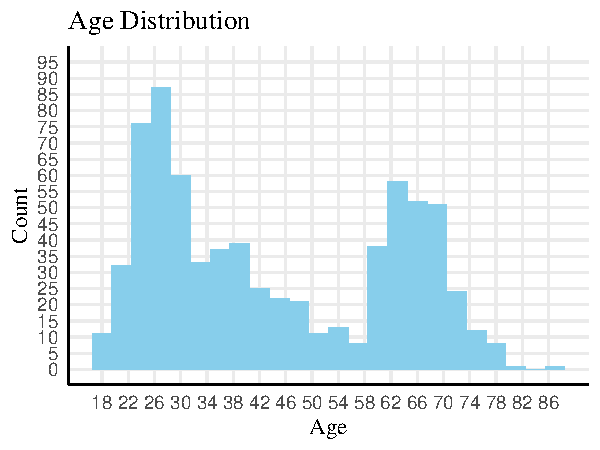
\includegraphics{Exploring-the-Role-of-Deviance-on-Self-Concept-Clarity-Across-the-Lifespan-_files/figure-latex/agedis-1.pdf}
\caption{\label{fig:agedis}Age Distrubition}
\end{figure}

\begin{table}[tbp]

\begin{center}
\begin{threeparttable}

\caption{\label{tab:matrix}Correlations Matrix for Self-Concept Clarity, Subjective Well-Being, and Life Marker Scale Across Age}

\begin{tabular}{lllllll}
\toprule
 & \multicolumn{1}{c}{SWLScr} & \multicolumn{1}{c}{SCCScr} & \multicolumn{1}{c}{MYA\%} & \multicolumn{1}{c}{MMA\%} & \multicolumn{1}{c}{MEA\%} & \multicolumn{1}{c}{Age}\\
\midrule
SWLScr & 1.00 & 0.36 & 0.37 & 0.37 & 0.30 & 0.09\\
SCCScr & 0.36 & 1.00 & 0.41 & 0.34 & 0.35 & 0.38\\
MYA\% & 0.37 & 0.41 & 1.00 & 0.77 & 0.61 & 0.60\\
MMA\% & 0.37 & 0.34 & 0.77 & 1.00 & 0.69 & 0.56\\
MEA\% & 0.30 & 0.35 & 0.61 & 0.69 & 1.00 & 0.61\\
Age & 0.09 & 0.38 & 0.60 & 0.56 & 0.61 & 1.00\\
\bottomrule
\addlinespace
\end{tabular}

\begin{tablenotes}[para]
\normalsize{\textit{Note.} SWL = Satisfaction with Life Scale, SCC = Self-Concept Clairty Scale, YA = Life Marker Scale's Young Adult items score, MA = Life Marker Scale's Middle-age Adult items score, EA = Life Marker Scale's Elderly Adult items score}
\end{tablenotes}

\end{threeparttable}
\end{center}

\end{table}

To test Hypothesis 1 and 2, I run a correlational analysis on Satisfaction with Life Scale, Self-Concept Clarity Scale, Life Marker Scale, and age, see in Table \ref{tab:matrix}. We found a significant positive association between self-concept clarity and satisfaction with life and all three age group's life marker degree of deviance positively associates with satisfaction with life.

I further explored if age groups will influence the relationship between self-concept clarity and satisfaction with life (see Figure \ref{fig:SCCtoSWL}).

\begin{figure}
\centering
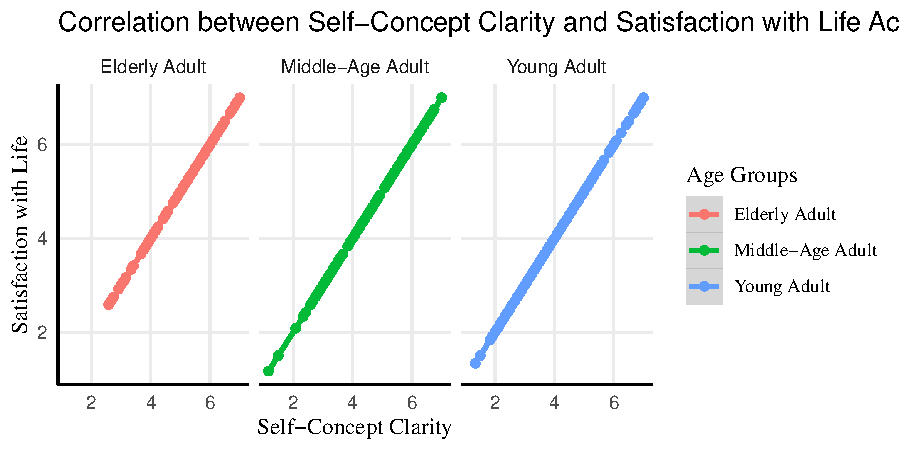
\includegraphics{Exploring-the-Role-of-Deviance-on-Self-Concept-Clarity-Across-the-Lifespan-_files/figure-latex/SCCtoSWL-1.pdf}
\caption{\label{fig:SCCtoSWL}Correlation between Self-Concept Clarity and Satisfaction with Life Across Age}
\end{figure}

\hypertarget{discussion}{%
\section{Discussion}\label{discussion}}

The analysis provided evidence for Hypothesis 1 and 2 that self-concept clarity and degree of deviance from the social clock have a positive association with subjective well-being. More specifically, people with greater self-concept clarity experience higher life satisfaction, and people who perceive themselves less deviant from the social clock have higher life satisfaction.

This study is significant because at the current stage of research, the underlying mechanism of the curvilinear relationship between self-concept clarity and subjective well-being is still open to interpretation. This study explores potential influential lifetime factors from a perspective which no research has explored before. Deviance from social clock, even though an older topic, may be able to bring new insight into different fields of research like self-concept clarity. With a more holistic perspective, it make sense trying to explain the curvilinear relationship with perceived deviance from the social clock.

However, this study is not without limitation. Since there is no existing scale measure deviance from the social clock, the measurement has no previous reliability or validity check. The measure itself can be difficult to develop due to very minimal research in this field on elderly adults' life markers. Thus, it can be hard to balance the number of markers for each age range.
Future studies can work on creating a more valid and reliable measurement for this concept, or knit the measurement for life markers, life satisfaction, self-concept clarity, self-esteem, etc. together for a holistic measurement aiming to capture the level of happiness in life.

\newpage

\hypertarget{references}{%
\section{References}\label{references}}

\hypertarget{refs}{}
\begin{CSLReferences}{1}{0}
\leavevmode\vadjust pre{\hypertarget{ref-abramsUnmetExpectationsWork2022}{}}%
Abrams, L. R., Clarke, P. J., \& Mehta, N. K. (2022). Unmet {Expectations About Work} at {Age} 62 and {Depressive Symptoms}. \emph{The Journals of Gerontology: Series B}, \emph{77}(3), 615--625. \url{https://doi.org/10.1093/geronb/gbab113}

\leavevmode\vadjust pre{\hypertarget{ref-arnettConceptionsTransitionAdulthood2001}{}}%
Arnett, J. J. (2001). Conceptions of the {Transition} to {Adulthood}: {Perspectives From Adolescence Through Midlife}. \emph{Journal of Adult Development}, \emph{8}(2), 133--143. \url{https://doi.org/10.1023/A:1026450103225}

\leavevmode\vadjust pre{\hypertarget{ref-R-papaja}{}}%
Aust, F., \& Barth, M. (2023). \emph{{papaja}: {Prepare} reproducible {APA} journal articles with {R Markdown}}. Retrieved from \url{https://github.com/crsh/papaja}

\leavevmode\vadjust pre{\hypertarget{ref-R-magrittr}{}}%
Bache, S. M., \& Wickham, H. (2022). \emph{Magrittr: A forward-pipe operator for r}. Retrieved from \url{https://CRAN.R-project.org/package=magrittr}

\leavevmode\vadjust pre{\hypertarget{ref-R-tinylabels}{}}%
Barth, M. (2023). \emph{{tinylabels}: Lightweight variable labels}. Retrieved from \url{https://cran.r-project.org/package=tinylabels}

\leavevmode\vadjust pre{\hypertarget{ref-R-lme4}{}}%
Bates, D., Mächler, M., Bolker, B., \& Walker, S. (2015). Fitting linear mixed-effects models using {lme4}. \emph{Journal of Statistical Software}, \emph{67}(1), 1--48. \url{https://doi.org/10.18637/jss.v067.i01}

\leavevmode\vadjust pre{\hypertarget{ref-R-Matrix}{}}%
Bates, D., Maechler, M., \& Jagan, M. (2023). \emph{Matrix: Sparse and dense matrix classes and methods}. Retrieved from \url{https://CRAN.R-project.org/package=Matrix}

\leavevmode\vadjust pre{\hypertarget{ref-blanchflowerHappinessUshapedEverywhere2021}{}}%
Blanchflower, D. G. (2021). Is happiness {U-shaped} everywhere? {Age} and subjective well-being in 145 countries. \emph{Journal of Population Economics}, \emph{34}(2), 575--624. \url{https://doi.org/10.1007/s00148-020-00797-z}

\leavevmode\vadjust pre{\hypertarget{ref-campbellSelfesteemClaritySelfconcept1990}{}}%
Campbell, J. D. (1990). Self-esteem and clarity of the self-concept. \emph{Journal of Personality and Social Psychology}, \emph{59}(3), 538--549. \url{https://doi.org/10.1037/0022-3514.59.3.538}

\leavevmode\vadjust pre{\hypertarget{ref-campbellStructureSelfConceptIts2003}{}}%
Campbell, J. D., Assanand, S., \& Paula, A. D. (2003). The {Structure} of the {Self-Concept} and {Its Relation} to {Psychological Adjustment}. \emph{Journal of Personality}, \emph{71}(1), 115--140. \url{https://doi.org/10.1111/1467-6494.t01-1-00002}

\leavevmode\vadjust pre{\hypertarget{ref-campbellSelfconceptClarityMeasurement1996}{}}%
Campbell, J. D., Trapnell, P. D., Heine, S. J., Katz, I. M., Lavallee, L. F., \& Lehman, D. R. (1996). Self-concept clarity: {Measurement}, personality correlates, and cultural boundaries. \emph{Journal of Personality and Social Psychology}, \emph{70}(1), 141--156. \url{https://doi.org/10.1037/0022-3514.70.1.141}

\leavevmode\vadjust pre{\hypertarget{ref-carterExaminingRelationshipSelfPerceptions2019}{}}%
Carter, M. J., \& Bruene, S. (2019). Examining the {Relationship Between Self-Perceptions} of {Person}, {Role}, and {Social Identity Change} and {Self-Concept Clarity}. \emph{Imagination, Cognition and Personality}, \emph{38}(4), 425--451. \url{https://doi.org/10.1177/0276236618792267}

\leavevmode\vadjust pre{\hypertarget{ref-R-shiny}{}}%
Chang, W., Cheng, J., Allaire, J., Sievert, C., Schloerke, B., Xie, Y., \ldots{} Borges, B. (2023). \emph{Shiny: Web application framework for r}. Retrieved from \url{https://CRAN.R-project.org/package=shiny}

\leavevmode\vadjust pre{\hypertarget{ref-dienerSatisfactionLifeScale1985}{}}%
Diener, E., Emmons, R. A., Larsen, R. J., \& Griffin, S. (1985). The {Satisfaction With Life Scale}. \emph{Journal of Personality Assessment}, \emph{49}(1), 71--75. \url{https://doi.org/10.1207/s15327752jpa4901_13}

\leavevmode\vadjust pre{\hypertarget{ref-R-lubridate}{}}%
Grolemund, G., \& Wickham, H. (2011). Dates and times made easy with {lubridate}. \emph{Journal of Statistical Software}, \emph{40}(3), 1--25. Retrieved from \url{https://www.jstatsoft.org/v40/i03/}

\leavevmode\vadjust pre{\hypertarget{ref-R-Hmisc}{}}%
Harrell Jr, F. E. (2023). \emph{Hmisc: Harrell miscellaneous}. Retrieved from \url{https://CRAN.R-project.org/package=Hmisc}

\leavevmode\vadjust pre{\hypertarget{ref-helsonPersonalityPatternsAdherence1984}{}}%
Helson, R., Mitchell, V., \& Moane, G. (1984). Personality and patterns of adherence and nonadherence to the social clock. \emph{Journal of Personality and Social Psychology}, \emph{46}(5), 1079--1096. \url{https://doi.org/10.1037/0022-3514.46.5.1079}

\leavevmode\vadjust pre{\hypertarget{ref-lightSelfConceptClaritySelfRegulation2017}{}}%
Light, A. E. (2017). Self-{Concept Clarity}, {Self-Regulation}, and {Psychological Well-Being}. In J. Lodi-Smith \& K. G. DeMarree (Eds.), \emph{Self-{Concept Clarity}: {Perspectives} on {Assessment}, {Research}, and {Applications}} (pp. 177--193). {Cham}: {Springer International Publishing}. \url{https://doi.org/10.1007/978-3-319-71547-6_10}

\leavevmode\vadjust pre{\hypertarget{ref-lightUnpublishedData2024}{}}%
Light, A. E. (2024). \emph{Unpublished data}. Unpublished Data.

\leavevmode\vadjust pre{\hypertarget{ref-lightInsOutsSelf2013}{}}%
Light, A. E., \& Visser, P. S. (2013). The {Ins} and {Outs} of the {Self}: {Contrasting Role Exits} and {Role Entries} as {Predictors} of {Self-concept Clarity}. \emph{Self and Identity}.

\leavevmode\vadjust pre{\hypertarget{ref-lodi-smithGettingKnowMe2010}{}}%
Lodi-Smith, J., \& Roberts, B. W. (2010). Getting to {Know Me}: {Social Role Experiences} and {Age Differences} in {Self-Concept Clarity During Adulthood}. \emph{Journal of Personality}, \emph{78}(5), 1383--1410. \url{https://doi.org/10.1111/j.1467-6494.2010.00655.x}

\leavevmode\vadjust pre{\hypertarget{ref-lopezulloaHowDoesSubjective2013}{}}%
López Ulloa, B. F., Møller, V., \& Sousa-Poza, A. (2013). How {Does Subjective Well-Being Evolve} with {Age}? {A Literature Review}. \emph{Journal of Population Ageing}, \emph{6}(3), 227--246. \url{https://doi.org/10.1007/s12062-013-9085-0}

\leavevmode\vadjust pre{\hypertarget{ref-R-correlationArticle}{}}%
Makowski, D., Ben-Shachar, M. S., Patil, I., \& Lüdecke, D. (2020). Methods and algorithms for correlation analysis in {R}. \emph{Journal of Open Source Software}, \emph{5}(51), 2306. \url{https://doi.org/10.21105/joss.02306}

\leavevmode\vadjust pre{\hypertarget{ref-R-tibble}{}}%
Müller, K., \& Wickham, H. (2023). \emph{Tibble: Simple data frames}. Retrieved from \url{https://CRAN.R-project.org/package=tibble}

\leavevmode\vadjust pre{\hypertarget{ref-neugartenTimeAgeLife1979}{}}%
Neugarten, B. L. (1979). Time, age, and the life cycle. \emph{The American Journal of Psychiatry}, \emph{136}(7), 887--894. \url{https://doi.org/10.1176/ajp.136.7.887}

\leavevmode\vadjust pre{\hypertarget{ref-pekel-uludagliYoungAdultsPerceptions2019}{}}%
Pekel-Uludağlı, N., \& Akbaş, G. (2019). Young {Adults}' {Perceptions} of {Social Clock} and {Adulthood Roles} in the {Turkish Population}. \emph{Journal of Adult Development}, \emph{26}(2), 105--115. \url{https://doi.org/10.1007/s10804-018-9298-9}

\leavevmode\vadjust pre{\hypertarget{ref-R-base}{}}%
R Core Team. (2023). \emph{R: A language and environment for statistical computing}. Vienna, Austria: R Foundation for Statistical Computing. Retrieved from \url{https://www.R-project.org/}

\leavevmode\vadjust pre{\hypertarget{ref-ritchieSelfconceptClarityMediates2011}{}}%
Ritchie, T. D., Sedikides, C., Wildschut, T., Arndt, J., \& Gidron, Y. (2011). Self-concept {Clarity Mediates} the {Relation} between {Stress} and {Subjective Well-being}. \emph{Self and Identity}, \emph{10}(4), 493--508. \url{https://doi.org/10.1080/15298868.2010.493066}

\leavevmode\vadjust pre{\hypertarget{ref-rookTimingMajorLife1989}{}}%
Rook, K. S., Catalano, R., \& Dooley, D. (1989). The timing of major life events: {Effects} of departing from the social clock. \emph{American Journal of Community Psychology}, \emph{17}(2), 233--258. \url{https://doi.org/10.1007/BF00931009}

\leavevmode\vadjust pre{\hypertarget{ref-slotterAllRoleTransitions2017}{}}%
Slotter, E., \& Walsh, C. (2017). All role transitions are not experienced equally: {Associations} among self-change, emotional reactions, and self-concept clarity. \emph{Self and Identity}, \emph{16}, 1--26. \url{https://doi.org/10.1080/15298868.2017.1280528}

\leavevmode\vadjust pre{\hypertarget{ref-stopaConstructingSelfRole2010}{}}%
Stopa, L., Brown, M. A., Luke, M. A., \& Hirsch, C. R. (2010). Constructing a self: {The} role of self-structure and self-certainty in social anxiety. \emph{Behaviour Research and Therapy}, \emph{48}(10), 955--965. \url{https://doi.org/10.1016/j.brat.2010.05.028}

\leavevmode\vadjust pre{\hypertarget{ref-R-ggplot2}{}}%
Wickham, H. (2016). \emph{ggplot2: Elegant graphics for data analysis}. Springer-Verlag New York. Retrieved from \url{https://ggplot2.tidyverse.org}

\leavevmode\vadjust pre{\hypertarget{ref-R-forcats}{}}%
Wickham, H. (2023a). \emph{Forcats: Tools for working with categorical variables (factors)}. Retrieved from \url{https://CRAN.R-project.org/package=forcats}

\leavevmode\vadjust pre{\hypertarget{ref-R-stringr}{}}%
Wickham, H. (2023b). \emph{Stringr: Simple, consistent wrappers for common string operations}. Retrieved from \url{https://CRAN.R-project.org/package=stringr}

\leavevmode\vadjust pre{\hypertarget{ref-R-tidyverse}{}}%
Wickham, H., Averick, M., Bryan, J., Chang, W., McGowan, L. D., François, R., \ldots{} Yutani, H. (2019). Welcome to the {tidyverse}. \emph{Journal of Open Source Software}, \emph{4}(43), 1686. \url{https://doi.org/10.21105/joss.01686}

\leavevmode\vadjust pre{\hypertarget{ref-R-dplyr}{}}%
Wickham, H., François, R., Henry, L., Müller, K., \& Vaughan, D. (2023). \emph{Dplyr: A grammar of data manipulation}. Retrieved from \url{https://CRAN.R-project.org/package=dplyr}

\leavevmode\vadjust pre{\hypertarget{ref-R-purrr}{}}%
Wickham, H., \& Henry, L. (2023). \emph{Purrr: Functional programming tools}. Retrieved from \url{https://CRAN.R-project.org/package=purrr}

\leavevmode\vadjust pre{\hypertarget{ref-R-readr}{}}%
Wickham, H., Hester, J., \& Bryan, J. (2024). \emph{Readr: Read rectangular text data}. Retrieved from \url{https://CRAN.R-project.org/package=readr}

\leavevmode\vadjust pre{\hypertarget{ref-R-haven}{}}%
Wickham, H., Miller, E., \& Smith, D. (2023). \emph{Haven: Import and export 'SPSS', 'stata' and 'SAS' files}. Retrieved from \url{https://CRAN.R-project.org/package=haven}

\leavevmode\vadjust pre{\hypertarget{ref-R-scales}{}}%
Wickham, H., Pedersen, T. L., \& Seidel, D. (2023). \emph{Scales: Scale functions for visualization}. Retrieved from \url{https://CRAN.R-project.org/package=scales}

\leavevmode\vadjust pre{\hypertarget{ref-R-tidyr}{}}%
Wickham, H., Vaughan, D., \& Girlich, M. (2023). \emph{Tidyr: Tidy messy data}. Retrieved from \url{https://CRAN.R-project.org/package=tidyr}

\leavevmode\vadjust pre{\hypertarget{ref-R-psych}{}}%
William Revelle. (2023). \emph{Psych: Procedures for psychological, psychometric, and personality research}. Evanston, Illinois: Northwestern University. Retrieved from \url{https://CRAN.R-project.org/package=psych}

\leavevmode\vadjust pre{\hypertarget{ref-R-knitr}{}}%
Xie, Y. (2015). \emph{Dynamic documents with {R} and knitr} (2nd ed.). Boca Raton, Florida: Chapman; Hall/CRC. Retrieved from \url{https://yihui.org/knitr/}

\leavevmode\vadjust pre{\hypertarget{ref-R-kableExtra}{}}%
Zhu, H. (2024). \emph{kableExtra: Construct complex table with 'kable' and pipe syntax}. Retrieved from \url{http://haozhu233.github.io/kableExtra/}

\end{CSLReferences}


\end{document}
